% !TEX program = xelatex
% !TEX TS-program = xelatex
% 컴파일: XeLaTeX (Overleaf: Menu > Compiler > XeLaTeX). 숫자는 numbers.tex, 표는 tables/, 그림은 figures/ 에서 자동으로 들어옴.
\documentclass[conference,a4paper]{IEEEtran}
\usepackage{fontspec}
\IfFileExists{kotex.sty}{\usepackage{kotex}}{\usepackage{xetexko}}
\IfFontExistsTF{TeX Gyre Termes}{\setmainfont{TeX Gyre Termes}}{}
\IfFontExistsTF{Noto Serif CJK KR}{\setmainhangulfont{Noto Serif CJK KR}}{%
  \IfFontExistsTF{Batang}{\setmainhangulfont{Batang}}{%
    \IfFontExistsTF{NanumMyeongjo}{\setmainhangulfont{NanumMyeongjo}}{%
      \IfFontExistsTF{AppleMyungjo}{\setmainhangulfont{AppleMyungjo}}{}}}}
\usepackage{amsmath,amssymb}
\usepackage{graphicx}
\usepackage{float}
\raggedbottom
\usepackage{booktabs}
\usepackage{xcolor}
\usepackage{tikz}
\usetikzlibrary{arrows.meta,positioning}
\usepackage[hidelinks]{hyperref}
\graphicspath{{figures/}}
% generated by 11_paper_assets.py - do not edit; re-run the pipeline instead
\newcommand{\FirstSeason}{1979-80}
\newcommand{\LastSeason}{2025-26}
\newcommand{\NSeasons}{47}
\newcommand{\NPages}{683}
\newcommand{\NPlayerRows}{25{,}349}
\newcommand{\NTeamSeasons}{1{,}314}
\newcommand{\NGames}{52{,}848}
\newcommand{\NPrimePlayers}{989}
\newcommand{\RhoOneThree}{0.94}
\newcommand{\RhoThreeFive}{0.96}
\newcommand{\RmseBPM}{3.00}
\newcommand{\RmseWS}{3.25}
\newcommand{\RmsePER}{3.44}
\newcommand{\RmseBox}{3.81}
\newcommand{\RmseBaseline}{3.72}
\newcommand{\MvpTopThreeBPM}{85\%}
\newcommand{\NbaTopTenBPM}{84\%}
\newcommand{\MvpTopThreePTS}{55\%}
\newcommand{\JordanBPM}{+12.0}
\newcommand{\JordanPTS}{33.7}
\newcommand{\JordanTS}{0.608}
\newcommand{\JordanLeagueTS}{0.535}
\newcommand{\JordanBPMRanks}{1, 1, 1}
\newcommand{\TopPrime}{Nikola Jokić}
\newcommand{\TopPrimeBPM}{+13.5}
\newcommand{\KUsage}{0.28}
\newcommand{\RmseTeamModel}{2.87}
\newcommand{\RTwoTeamModel}{0.66}
\newcommand{\RmseRidge}{2.68}
\newcommand{\BestRealTeam}{CHI 1995-96}
\newcommand{\BestRealNR}{+13.4}
\newcommand{\HomeCourt}{1.74}
\newcommand{\SigmaGame}{14.05}
\newcommand{\BrierTest}{0.208}
\newcommand{\Coverage}{93.3\%}
\newcommand{\NFives}{976{,}952}
\newcommand{\PriceOfPositions}{0.8}
\newcommand{\NSims}{100{,}000}
\newcommand{\NLeagueSeasons}{1{,}180{,}000}
\newcommand{\NLeagueGames}{1{,}451{,}400{,}000}
\newcommand{\NHtoH}{4{,}800{,}000}
\newcommand{\ReplacedTeam}{Washington Wizards}
\newcommand{\BestLabel}{B}
\newcommand{\BestFive}{Chris Paul, Michael Jordan, LeBron James, Giannis Antetokounmpo, Nikola Jokić}
\newcommand{\BestRating}{+33.0}
\newcommand{\BestMeanWins}{80.4}
\newcommand{\BestTitleOdds}{99.9\%}
\newcommand{\BestTitleOddsUnc}{99.8\%}
\newcommand{\BestMinGameWin}{90\%}
\newcommand{\BestMaxGameWin}{97\%}
\newcommand{\BestVsBullsGame}{90\%}
\newcommand{\BoostingTitleOdds}{10.5\%}

% generated by 13_all_time_teams.py - do not edit; re-run the script instead
\newcommand{\FirstTeamNames}{Chris Paul, Michael Jordan, LeBron James, Giannis Antetokounmpo, Nikola Jokić}
\newcommand{\FirstTeamRating}{+33.0}
\newcommand{\FirstTeamWins}{80.4}
\newcommand{\FirstTeamWinsRange}{78--82}
\newcommand{\FirstTeamPerfect}{18.9\%}
\newcommand{\FirstTeamTitle}{99.9\%}
\newcommand{\FirstTeamTitleUnc}{99.8\%}
\newcommand{\FirstTeamDynGame}{94\%}
\newcommand{\FirstTeamDynGameMin}{90\%}
\newcommand{\FirstTeamDynGameMax}{97\%}
\newcommand{\FirstTeamBullsSeries}{99.8\%}
\newcommand{\SecondTeamNames}{Shai Gilgeous-Alexander, Magic Johnson, Kevin Durant, Jimmy Butler, David Robinson}
\newcommand{\SecondTeamRating}{+28.7}
\newcommand{\SecondTeamWins}{78.9}
\newcommand{\SecondTeamWinsRange}{76--81}
\newcommand{\SecondTeamPerfect}{4.2\%}
\newcommand{\SecondTeamTitle}{99.5\%}
\newcommand{\SecondTeamTitleUnc}{99.1\%}
\newcommand{\SecondTeamDynGame}{90\%}
\newcommand{\SecondTeamDynGameMin}{84\%}
\newcommand{\SecondTeamDynGameMax}{95\%}
\newcommand{\SecondTeamBullsSeries}{98.6\%}
\newcommand{\ThirdTeamNames}{John Stockton, Manu Ginóbili, Kawhi Leonard, Kevin Garnett, Anthony Davis}
\newcommand{\ThirdTeamRating}{+24.5}
\newcommand{\ThirdTeamWins}{76.7}
\newcommand{\ThirdTeamWinsRange}{73--80}
\newcommand{\ThirdTeamPerfect}{0.4\%}
\newcommand{\ThirdTeamTitle}{97.4\%}
\newcommand{\ThirdTeamTitleUnc}{96.1\%}
\newcommand{\ThirdTeamDynGame}{85\%}
\newcommand{\ThirdTeamDynGameMin}{77\%}
\newcommand{\ThirdTeamDynGameMax}{91\%}
\newcommand{\ThirdTeamBullsSeries}{94.5\%}
\newcommand{\PickTeamNames}{Stephen Curry, Michael Jordan, LeBron James, Larry Bird, David Robinson}
\newcommand{\PickTeamRating}{+28.7}
\newcommand{\PickTeamWins}{78.9}
\newcommand{\PickTeamWinsRange}{76--81}
\newcommand{\PickTeamPerfect}{4.3\%}
\newcommand{\PickTeamTitle}{99.5\%}
\newcommand{\PickTeamTitleUnc}{99.1\%}
\newcommand{\PickTeamDynGame}{90\%}
\newcommand{\PickTeamDynGameMin}{84\%}
\newcommand{\PickTeamDynGameMax}{95\%}
\newcommand{\PickTeamBullsSeries}{98.6\%}
\newcommand{\FirstVsSecondGame}{62\%}
\newcommand{\FirstVsSecondSeries}{74\%}
\newcommand{\FirstVsThirdGame}{72\%}
\newcommand{\FirstVsThirdSeries}{90\%}
\newcommand{\SecondVsThirdGame}{61\%}
\newcommand{\SecondVsThirdSeries}{74\%}
\newcommand{\FirstVsPickGame}{62\%}
\newcommand{\FirstVsPickSeries}{74\%}
\newcommand{\NAllTimeSeasons}{800{,}000}
\newcommand{\NAllTimeGames}{6{,}000{,}000}

\newcommand{\note}[1]{{\color{gray}\itshape [Notes: #1]}}

\begin{document}

\title{통계 모델링과 몬테카를로 시뮬레이션을 이용한\\NBA 역대 All-NBA 팀 선정\\[6pt]
{\Large (Selecting the NBA's All-Time All-NBA Teams Using Statistical Modeling and Monte Carlo Simulation)\par}}

\author{\IEEEauthorblockN{최재원 (Jaewon Choi)}
\IEEEauthorblockA{서울대학교 컴퓨터공학 \\ just\_aoj@snu.ac.kr \\ https://github.com/justaoj}}

\maketitle

\section{서론}
(한국어로 문서를 작성하는 게 익숙지 않아서 이상하거나 잘 읽히지 않는 부분이 있더라도 양해 부탁드립니다.)\\

이번 중간 과제가 `본인의 전공과 농구를 융합하여 아이디어 만들어 보기'여서, 제 주전공인 컴퓨터공학과 농구를 융합해 할 수 있는 것이 무엇이 있을까 생각하다가 나온 것이 바로 농구 팬들 사이에서 끝나지 않는 ``역대 최강 팀'' 논쟁을 데이터와 시뮬레이션으로 분석해 보는 과제였습니다.\\

저는 해외에서 쭉 거주했기 때문에 중학생 때부터 NBA를 보아 왔습니다. 중학교 때까지 학교 농구 팀에서 뛸 정도로 농구를 많이 좋아했는데, 친구들과 NBA를 보면서 당시 자주 하던 논쟁이 `역대 최고의 선수, 팀은 누구인가'였습니다. 사람마다 좋아하는 선수나 중요하게 생각하는 지표가 달라서 재미난 논쟁거리가 되곤 했습니다.\\

그래서 이번 과제를 기회로, 컴퓨터공학을 전공하며 배운 데이터 수집, 모델 검증, 탐색 알고리즘, 시뮬레이션을 이 논쟁에 적용할 수 있다고 보고 이번 과제의 주제로 정하였습니다. 연구 질문은 다음과 같습니다: 3점슛이 도입된 1979--80 시즌 이후의 선수 중 올-NBA 팀처럼 가드 2명, 포워드 2명, 센터 1명을 고른다면 통계적으로 가장 강한 다섯은 누구이며, 그 팀은 실제 리그와 역대 왕조를 상대로 얼마나 이기는가?\\

이를 위해 본 연구는 (1) 선수 평가 지표의 정확도를 예측 성능으로 검증하고, (2) 다섯 명이 공 하나를 사용률 비율에 맞춰 나눠 쓴다는 가정하에 팀 모델을 만들고, (3) 가능한 모든 라인업을 탐색한 후, (4) 경기·시리즈·시즌 단위로 몬테카를로 시뮬레이션을 수행했습니다. 전체 흐름은 \ref{sec:pipeline}절에서 더 자세히 설명합니다.

% =====================================================================
\section{모델 파이프라인}\label{sec:pipeline}
Figure~\ref{fig:pipeline}은 모델의 전체 흐름입니다. 모든 단계는 Python(pandas, scikit-learn~\cite{sklearn})으로 작성한 스크립트이며, 데이터가 바뀌더라도 한 번의 실행으로 모든 표와 그림이 다시 만들어지는 구조로 만들었습니다. 모든 시뮬레이션과 그래프 제작은 제 컴퓨터의 로컬 IDE에서 진행되었습니다(코드는 제 GitHub에서 찾아볼 수 있습니다).\\

우선 데이터 수집 단계에서는 NBA 관련 수치와 통계를 기록해 둔 Basketball-Reference에서 웹페이지 \NPages{}개를 다운로드했습니다(\ref{sec:data}절). 파싱 단계에서는 이를 선수-시즌 \NPlayerRows{}행, 팀-시즌 \NTeamSeasons{}개, 경기 \NGames{}개의 표로 바꾸었으며, 이 중 규정 출전 시즌이 3시즌 이상 이어진 \NPrimePlayers{}명이 분석 대상이었습니다. 지표 검증 단계에서는 어떤 선수 지표가 팀 성적을 가장 잘 예측하는지 비교하여 최종적으로 BPM을 선택했습니다(\ref{sec:bpm}절). 팀 모델 단계에서는 원볼 사용률(one-ball usage) 모델로, 다섯 명이 공 하나를 사용률 비율에 맞춰 나눠 쓴다고 가정하고 다섯 명의 조합을 하나의 팀 실력, 즉 넷레이팅(100포세션당 득실차)으로 바꿨습니다(\ref{sec:onebal}절). 마지막으로 라인업 탐색 단계에서는 BPM 상위 60명으로 만들 수 있는 G-G-F-F-C 조합 \NFives{}개를 모두 평가했습니다. 이를 통해 사람의 편견 없이 수치만으로 판단한 최고의 팀이 완성됩니다.\\

마지막 단계는 몬테카를로 시뮬레이션입니다. 몬테카를로 시뮬레이션은 결과를 한 번의 계산으로 구하기 어려울 때, 같은 상황을 컴퓨터로 수없이 반복해 보고 그 결과를 모아 확률을 구하는 방법입니다~\cite{mc}. 예를 들어, 동전을 10만 번 던져 앞면이 나온 횟수를 세면, 앞면이 나올 확률이 약 50\%라는 것을 알 수 있는 원리와 같습니다.\\

이 연구에서는 같은 원리를 농구 시즌에 적용했습니다. 먼저 두 팀의 실력 차이로 한 경기의 승리 확률을 정하고, 컴퓨터가 그 확률에 맞춰 경기마다 승패를 무작위로 정합니다. 이렇게 정규시즌 82경기부터 플레이오프까지 한 시즌을 끝까지 진행하는 것을 10만 번 반복한 뒤, 그중 우승한 시즌의 비율을 우승 확률로 사용했습니다.

\begin{figure}[!h]
\centering
\begin{tikzpicture}[
  box/.style={draw, rounded corners=2pt, align=center, font=\scriptsize, minimum width=2.3cm, minimum height=1.25cm, inner sep=2pt},
  arr/.style={-{Stealth[length=4pt]}, semithick}]
\node[box] (d) {Data collection\\{\tiny (데이터 수집)}\\[1pt]{\tiny \NPages{} pages, 1979--2026}};
\node[box, right=0.28cm of d] (p) {Parsing \& cleaning\\{\tiny (파싱·정제)}\\[1pt]{\tiny \NPlayerRows{} player-seasons}};
\node[box, right=0.28cm of p] (m) {Metric validation\\{\tiny (선수 지표 검증)}\\[1pt]{\tiny BPM, cross-validation}};
\node[box, below=0.45cm of m] (t) {Team model\\{\tiny (팀 모델)}\\[1pt]{\tiny one-ball usage model}};
\node[box, left=0.28cm of t] (s) {Lineup search\\{\tiny (라인업 탐색)}\\[1pt]{\tiny \NFives{} lineups}};
\node[box, left=0.28cm of s, fill=blue!8] (mc) {Monte Carlo\\{\tiny (몬테카를로 시뮬레이션)}\\[1pt]{\tiny games, series, seasons}};
\draw[arr] (d) -- (p); \draw[arr] (p) -- (m); \draw[arr] (m) -- (t); \draw[arr] (t) -- (s); \draw[arr] (s) -- (mc);
\end{tikzpicture}
\caption{연구 파이프라인. 모든 단계는 Python 스크립트(01--13)로 구현되어 한 번에 재실행 가능.}
\label{fig:pipeline}
\end{figure}

% =====================================================================
\section{데이터}\label{sec:data}
데이터는 앞에서 설명한, NBA 기록을 정리해 제공하는 Basketball-Reference~\cite{bbref}에서 수집하였습니다. 기간은 \FirstSeason{}부터 \LastSeason{}까지 \NSeasons{}시즌입니다. 1979--80 시즌을 시작점으로 정한 이유는 이 시즌에 3점슛이 도입되었고 스틸·블록·턴오버가 모두 기록되어 BPM을 온전히 계산할 수 있기 때문입니다. 이전 시대 선수(윌트 체임벌린, 빌 러셀 등)는 기록 방식이 달라 같은 기준으로 비교할 수 없으므로, 본 연구에서 ``역대''는 3점슛 시대를 뜻합니다.\\

경기 수가 적었던 단축 시즌(1998--99, 2011--12, 2019--20, 2020--21)은 출전 시간 기준을 비례해 낮췄으며, 정규시즌 경기만 남기고 플레이인·플레이오프·인시즌 토너먼트 결승은 제외하였습니다. 한 시즌을 규정 출전으로 인정하는 기준은 82경기 기준 1{,}500분 이상입니다 (데이터 규모는 Table~\ref{tab:data}과 같습니다).

\begin{table}[t]
\centering
\caption{데이터 요약 (출처: Basketball-Reference)}
\label{tab:data}
\footnotesize
\setlength{\tabcolsep}{4pt}
\begin{tabular}{@{}lrl@{}}
\toprule
항목 & 개수 & 비고 \\
\midrule
다운로드한 웹페이지 & 683 & 시즌당 약 15쪽 \\
선수-시즌 행 & 25{,}349 & 트레이드 선수는 팀별 + 합계 행 \\
전성기(3년 기준) 선수 & 989 & 시즌당 1{,}500분 이상, 연속 3시즌 \\
팀-시즌 & 1{,}314 & 1979-80--2025-26 \\
정규시즌 경기 & 52{,}848 & 플레이인, 플레이오프, 컵 결승 제외 \\
\bottomrule
\end{tabular}
\end{table}


% =====================================================================
\section{All-Time All-NBA 팀 찾기}

\subsection{선수 평가 지표: BPM}\label{sec:bpm}
일단 선수를 평가하는 방법은 너무 많습니다. 예를 들어, 최근 화제가 된 ``82-0'' 게임은 득점·리바운드·어시스트·스틸·블록을 더한 값을 쓰고~\cite{game820}, PER은 분당 기록을 하나의 효율 점수로, Win Shares는 팀 승리에 대한 기여를 승수로 나타냅니다. 선수가 코트에 있을 때와 없을 때의 득실차를 회귀로 분리하는 RAPM~\cite{sill}과 이를 발전시킨 EPM, RAPTOR, LEBRON 같은 지표도 있지만, 이들은 플레이별(play-by-play) 기록이나 선수 추적 데이터가 필요해 1990년대 후반 이전 선수에게는 쓸 수 없습니다.\\

여러 방식을 고려한 끝에 저는 Box Plus/Minus(BPM)~\cite{bpm}을 사용했습니다. BPM은 박스스코어만으로 계산되므로 1979--80 이후 모든 시즌에 존재하고, 실제 득실차 데이터(RAPM)에 맞춰 만든 회귀식이며, 같은 시즌의 리그 평균 선수를 0으로 두므로 시대 차이가 일부 보정됩니다. 또한 \ref{sec:jordan}절의 검증에서 비교한 지표 중 가장 정확했기 때문에 채택했습니다.

\begin{equation}
\mathrm{BPM}_{\text{전성기}} = \frac{\sum_{s \in W} \mathrm{MP}_s \, \mathrm{BPM}_s}{\sum_{s \in W} \mathrm{MP}_s},\quad |W| = 3
\label{eq:prime}
\end{equation}

부가 설명을 하자면, BPM은 정확히는 각 선수의 100포세션당 박스스코어 기록에 가중치를 곱해 더한 값입니다. 포인트가드를 예로 들면 스틸 하나는 $+1.37$점, 턴오버 하나는 $-0.96$점의 가중치를 가지며, 가중치는 선수의 포지션과 공격 역할에 따라 달라집니다. 여기에 팀 보정을 더해, 한 팀 선수들의 출전 시간 가중 BPM 합이 그 팀의 실제 넷레이팅과 맞도록 합니다. 단위는 평균 선수 대비 100포세션당 득실이며, $+10$은 역대급 시즌, 0은 평균 수준의 선수를 뜻합니다. 공격 부분(OBPM)과 수비 부분(DBPM)을 더하면 BPM이 됩니다.\\

한 시즌 기록에는 운의 요소가 섞일 수 있으므로, 선수마다 가장 좋은 연속 3시즌을 전성기로 정하고 출전 시간으로 가중 평균하였습니다(수식~\eqref{eq:prime}). 예를 들어 마이클 조던의 경우 $(3311\times12.9 + 3255\times11.9 + 3197\times11.2)/9763 = +12.0$입니다 (참고로 이 방법을 \NPrimePlayers{}명에게 적용한 결과 1위는 \TopPrime{}(\TopPrimeBPM{})입니다(Figure~\ref{fig:primes})). 

\begin{figure}[t]
\centering
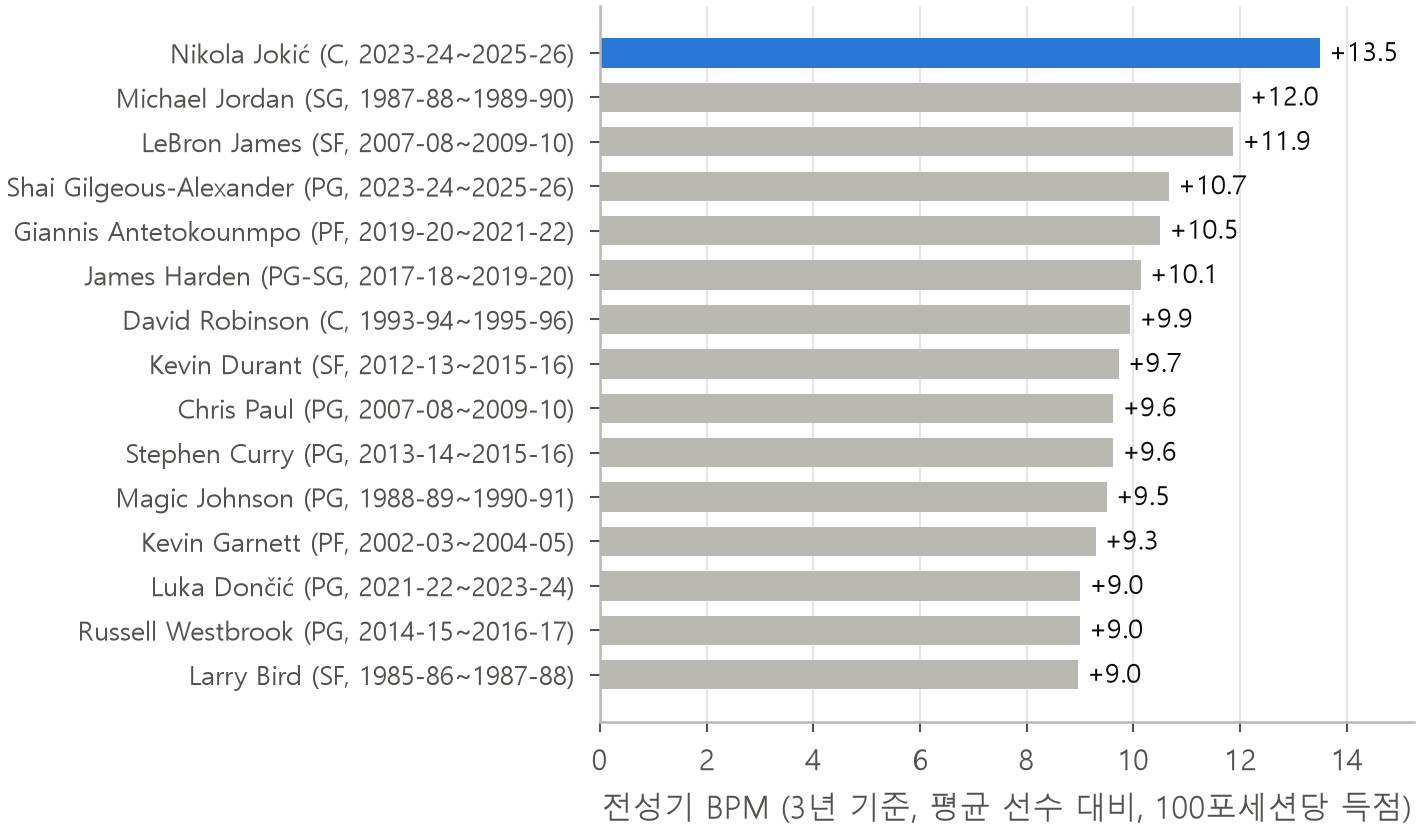
\includegraphics[width=\columnwidth]{fig5_top_primes.png}
\caption{전성기 BPM (3년 기준) 상위 15명 (\FirstSeason{}--\LastSeason{}). 괄호는 전성기 포지션과 기간.}
\label{fig:primes}
\end{figure}

\subsection{사례 연구: 마이클 조던과 지표의 정확도}\label{sec:jordan}
\begin{table}[!h]
\centering
\caption{마이클 조던 1987-88--1989-90 3시즌 기록과 리그 평균 (출전 시간 가중 평균)}
\label{tab:jordan}
\footnotesize
\begin{tabular}{@{}lrrr@{}}
\toprule
지표 & 마이클 조던 & 리그 평균 & 백분위 \\
\midrule
득점 PTS/G & 33.7 & 12.9 & 100 \\
TS\% & 0.608 & 0.535 & 93 \\
USG\% & 33.3 & 19.9 & 99 \\
AST\% & 30.1 & 15.1 & 89 \\
TRB\% & 9.9 & 10.0 & 51 \\
STL\% & 3.7 & 1.7 & 98 \\
BLK\% & 1.6 & 1.3 & 72 \\
TOV\% (낮을수록 좋음) & 10.4 & 14.4 & 84 \\
ORtg & 123.0 & 108.0 & 97 \\
PER & 31.3 & 15.0 & 100 \\
WS/48 & 0.295 & 0.101 & 100 \\
OBPM & 8.8 & 0.0 & 100 \\
DBPM & 3.2 & 0.0 & 99 \\
BPM & 12.0 & 0.0 & 100 \\
\bottomrule
\end{tabular}
\end{table}


\begin{figure}[!h]
\centering
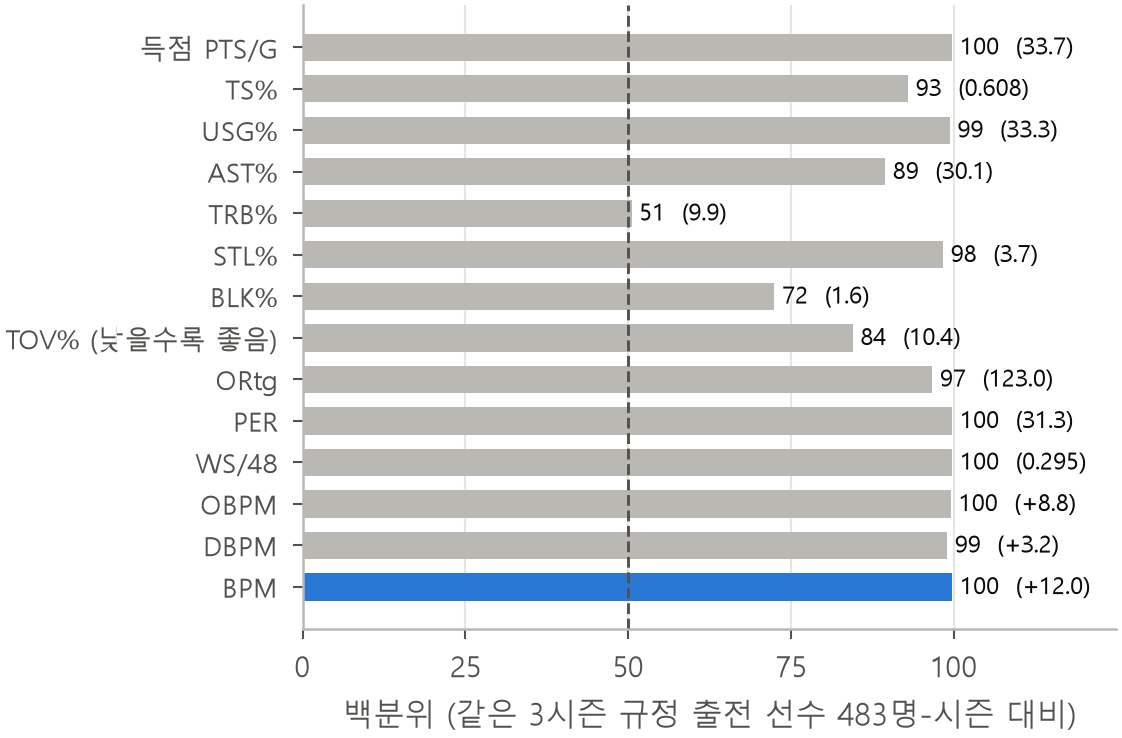
\includegraphics[width=\columnwidth]{fig4_jordan.png}
\caption{조던 전성기(3년 기준)의 지표별 백분위 (같은 3시즌 규정 출전 선수 대비). 괄호는 조던의 값.}
\label{fig:jordan}
\end{figure}

조던의 1987--88 $\sim$ 1989--90 전성기를 예로 여러 지표가 무엇을 말하는지 살펴보았습니다(Table~\ref{tab:jordan}, Figure~\ref{fig:jordan}). 조던은 이 기간 평균 \JordanPTS{}점을 넣으면서 슈팅 효율(TS\%) \JordanTS{}로 리그 평균 \JordanLeagueTS{}를 크게 넘었으며, BPM \JordanBPM{}으로 세 시즌 모두 리그 1위였습니다. 14개 지표 중 10개에서 상위 10\% 안에 들었고, 리바운드 비율만 리그 평균 수준이었는데, 이는 가드라는 포지션의 특성이라고 볼 수 있습니다. 처음 테스트를 할 때 고려하지 못했던 점인데, 이렇게 극단적으로 뛰어난 선수는 어떤 지표로 보아도 1위이므로 이번 사례 연구만으로는 어떤 지표가 정확한지 가릴 수 없었습니다. 그래서 모든 팀을 대상으로 예측 검증을 추가로 수행했습니다.


\begin{equation}
\widehat{\mathrm{NR}}_{t} = \alpha + \beta \sum_{i} s_i \, m_{i,t-1}, \qquad s_i = \frac{\mathrm{MP}_i}{\mathrm{MP}_{\text{team}}/5}
\label{eq:retro}
\end{equation}

추가 검증 방법은 다음과 같습니다. 각 팀-시즌에 대해 그 팀 선수들의 직전 시즌 지표를 출전 시간 비중으로 가중합하고(수식~\eqref{eq:retro}), 이 값으로 그 시즌의 팀 넷레이팅을 예측해 실제 값과 비교합니다. 오차의 크기는 RMSE(root mean square error, 평균 제곱근 오차)로 쟀습니다. RMSE는 예측이 실제에서 보통 몇 점 빗나가는지를 나타내며, 작을수록 정확하다는 뜻입니다.

\begin{figure}[!h]
\centering
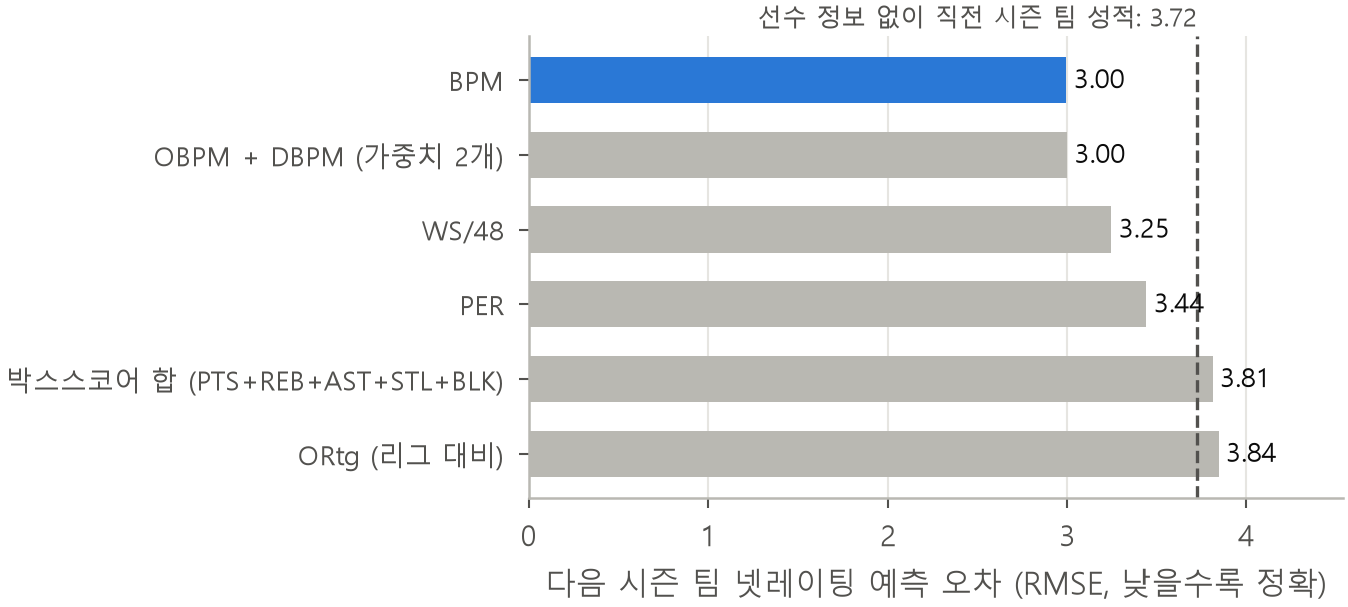
\includegraphics[width=\columnwidth]{fig2_metric_rmse.png}
\caption{지표별 다음 시즌 팀 넷레이팅 예측 오차 (교차검증 RMSE, \NTeamSeasons{}개 팀-시즌 중 직전 시즌이 있는 경우). 점선은 선수 정보 없이 직전 시즌 팀 성적만 쓴 기준선.}
\label{fig:rmse}
\end{figure}

결과는 Figure~\ref{fig:rmse}와 같습니다. BPM의 오차가 \RmseBPM{}으로 가장 작았고, WS/48 \RmseWS{}, PER \RmsePER{} 순이었습니다. 득점·리바운드 등을 더한 박스스코어 합은 \RmseBox{}로, 선수 정보 없이 직전 시즌 팀 성적만 쓴 기준선(\RmseBaseline{})보다도 나빴습니다. 기록을 단순히 더하는 방식으로는 팀 성적을 설명할 수 없다는 결론이 나왔습니다.

\begin{figure}[H]
\centering
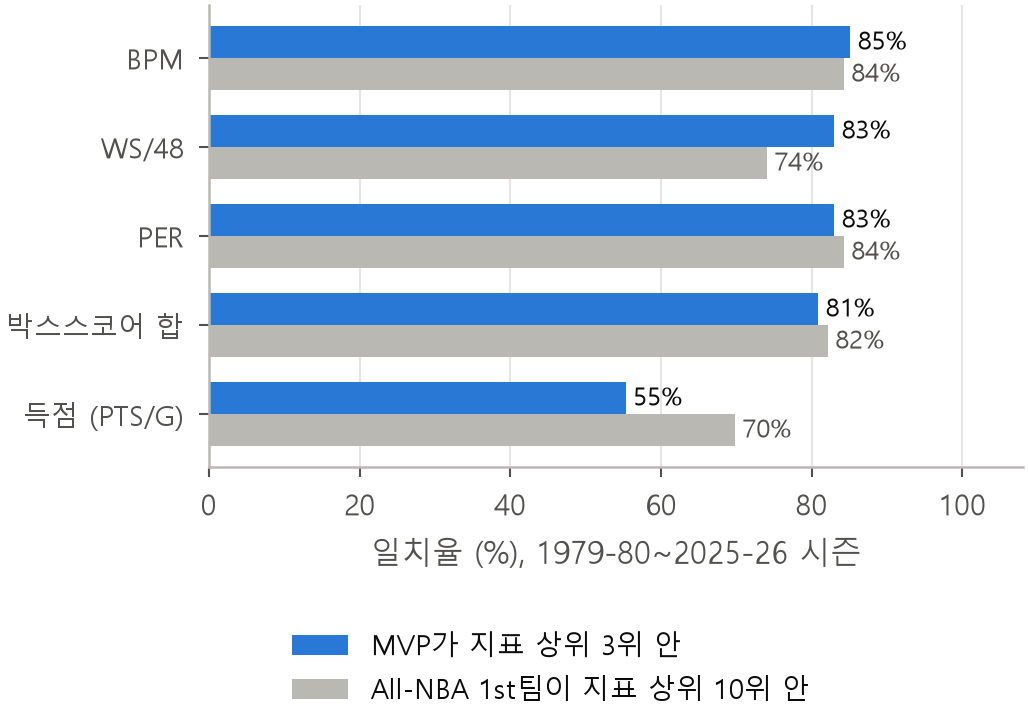
\includegraphics[width=0.8\columnwidth]{fig3_awards.png}
\caption{지표와 전문가 평가의 일치율. 파랑: MVP가 그 시즌 지표 상위 3위 안, 회색: All-NBA 1st팀 선수가 상위 10위 안.}
\label{fig:awards}
\end{figure}

전문가 평가와도 비교하였습니다(Figure~\ref{fig:awards}). MVP 수상자가 그 시즌 BPM 상위 3위 안에 든 비율은 \MvpTopThreeBPM{}로, 득점만 썼을 때(\MvpTopThreePTS{})보다 높았습니다. All-NBA 퍼스트 팀 선수가 BPM 상위 10위 안에 든 비율은 \NbaTopTenBPM{}였습니다. 다만 투표인단도 기록을 참고하므로 이 일치는 보조 근거이고, 주된 근거는 앞의 예측 검증입니다.


\subsection{팀 모델: 원볼(one-ball) 사용률 모델}\label{sec:onebal}
다섯 명의 스타를 한 팀에 모으면 공이 하나라는 문제가 생깁니다. 사용률(USG\%)은 선수가 코트에 있는 동안 팀 공격이 그 선수의 슛·자유투·턴오버로 끝나는 비율입니다~\cite{oliver,kubatko}. 퍼스트 팀 선수들은 각자의 팀에서 사용률 26--35\%를 기록했는데, 다섯 명을 더하면 157\%가 됩니다. 실제 팀의 사용률 합은 100\%이므로, BPM을 단순히 더한 값($+57.5$)은 다섯 명 모두가 원래 팀에서처럼 공을 쥔다고 가정한 셈입니다.\\

원볼 사용률 모델은 이 문제를 다음과 같이 처리합니다(수식~\eqref{eq:usage}, \eqref{eq:rating}). 먼저 다섯 명의 사용률을 합이 100\%가 되도록 비례해서 줄입니다. 공을 덜 쥐는 선수는 더 좋은 슛만 고를 수 있으므로 효율이 오르는데, 사용률을 1\%p 내줄 때마다 효율이 $k$만큼 오른다고 둡니다. 수비는 DBPM의 합으로 계산합니다.

\begin{gather}
u_i' = \frac{100\,u_i}{\sum_j u_j}, \qquad o_i' = o_i - k\,(u_i' - u_i) \label{eq:usage}\\
R = \frac{1}{100}\sum_i u_i' \, o_i' + \sum_i \mathrm{DBPM}_i \label{eq:rating}
\end{gather}
여기서 $u_i$는 사용률, $o_i$는 리그 평균 대비 공격 효율(ORtg $-$ 리그 평균), $R$은 팀 넷레이팅입니다.

$k$는 임의로 정한 값이 아니라 데이터에서 추정하였습니다. 두 시즌 연속 1{,}000분 이상 뛴 같은 선수의 시즌 쌍 8{,}353개(1{,}542명)에서 사용률 변화와 효율 변화 사이의 기울기를 구하면 $-0.28$이며, 따라서 $k=\KUsage{}$입니다. 서로 다른 선수끼리 비교하면 좋은 선수가 공도 많이 쥐고 효율도 높아 ``공을 많이 쥘수록 효율이 좋다''는 잘못된 관계가 보이지만, 같은 선수의 시즌끼리 비교하면 실력 차이가 사라지고 공을 더 쥐는 비용만 남습니다. 선수를 무작위로 다시 뽑아 200번 추정한 부트스트랩~\cite{efron}의 90\% 구간은 0.24--0.33입니다.\\

조던을 예로 들면, 퍼스트 팀에서 조던의 사용률은 33.3\%에서 21.2\%로 12.1\%p 줄고, 효율은 $0.28\times12.1 \approx +3.4$점 올라 리그 평균 대비 $+14.8$에서 $+18.2$가 됩니다. 다섯 명을 모두 계산하면 공격 $+16.4$, 수비 $+16.6$으로 팀 넷레이팅은 $+33.0$입니다. $k=0$이면 $+29.7$, $k=0.4$이면 $+34.3$입니다.\\

이 모델을 실제 \NTeamSeasons{}개 팀-시즌에 적용해 교차검증한 오차는 \RmseTeamModel{}($R^2$ \RTwoTeamModel{})이었고, 같은 특성을 쓴 릿지 회귀~\cite{ridge}(\RmseRidge{})와 비슷하였습니다(Figure~\ref{fig:team}). 실제 팀에서는 두 모델의 차이가 작지만, 사용률 합이 157\%인 올타임 팀은 실제 데이터의 범위를 크게 벗어납니다. 이런 팀에는 데이터에서만 배운 모델보다 공이 하나라는 규칙을 구조로 가진 모델이 더 안전하다고 판단하여 원볼 모델을 주 모델로 사용하였습니다.

\begin{figure}[H]
\centering
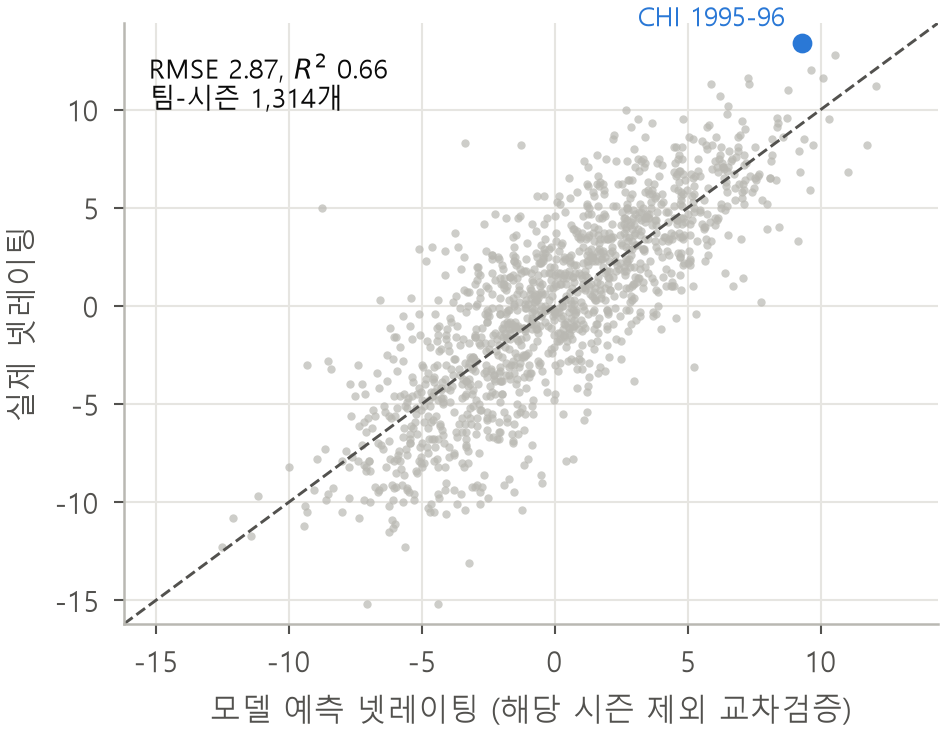
\includegraphics[width=\columnwidth]{fig6_team_model.png}
\caption{원볼 모델의 교차검증 예측 넷레이팅과 실제 넷레이팅 (\NTeamSeasons{}개 팀-시즌). 파란 점은 역대 최고 실제 팀 \BestRealTeam{} (\BestRealNR{}).}
\label{fig:team}
\end{figure}

\subsection{베스트 5 선정 방법 (G-G-F-F-C)}
팀 구성은 실제 올-NBA 팀처럼 가드(G) 2명, 포워드(F) 2명, 센터(C) 1명으로 하였습니다. 전성기 동안 PG 또는 SG로 등록된 선수는 G, SF 또는 PF로 등록된 선수는 F, C로 등록된 선수는 C 자리에 들어갈 수 있으며, 다섯 명이 자리에 맞게 배정되는지는 해당 알고리즘으로 확인합니다~\cite{kuhn}. 전성기 BPM 상위 60명으로 만들 수 있는 조합 \NFives{}개를 모두 원볼 모델로 평가해 가장 높은 조합을 퍼스트 팀으로 정하고, 그 다섯 명을 뺀 뒤 다시 탐색해 세컨드 팀을, 같은 방법으로 서드 팀을 정하였습니다.\\

TABLE~\ref{tab:candidates}(다음 페이지)은 같은 탐색에서 기준을 바꾼 후보들입니다. BPM 합이 가장 큰 다섯(A)은 원볼 모델 기준으로 최적 조합(B)보다 낮습니다. 두 팀은 두 번째 가드 한 자리만 다른데, 수비 수치가 좋은 크리스 폴이 셰이 길저스-알렉산더보다 조합에 더 잘 맞습니다. 박스스코어 합이 가장 큰 다섯(C)과 흔히 거론되는 팬 선정 다섯(D)은 그보다 낮습니다.

\begin{table*}[t]
\centering
\caption{후보 라인업과 시뮬레이션 결과 (경기·시리즈·시즌 각 100{,}000회)}
\label{tab:candidates}
\footnotesize
\setlength{\tabcolsep}{4pt}
\begin{tabular}{@{}clllllrrrrr@{}}
\toprule
팀 & G & G & F & F & C & 넷레이팅 & \shortstack{왕조 상대\\경기 승률} & \shortstack{1995--96 불스\\상대 시리즈} & \shortstack{정규시즌 승수\\{[}90\% 구간{]}} & \shortstack{우승 확률\\(불확실성 포함)} \\
\midrule
A & Gilgeous-Alexander & Jordan & James & Antetokounmpo & Jokić & +32.8 & 94.1\% & 99.8\% & 80.3 [78--82] & 99.9\% (99.8\%) \\
B & Paul & Jordan & James & Antetokounmpo & Jokić & +33.0 & 94.2\% & 99.8\% & 80.4 [78--82] & 99.9\% (99.8\%) \\
C & Dončić & Jordan & James & Antetokounmpo & Jokić & +29.5 & 91.0\% & 98.9\% & 79.3 [76--82] & 99.7\% (99.3\%) \\
D & Johnson & Jordan & James & Duncan & O'Neal & +26.8 & 87.9\% & 97.3\% & 78.1 [75--81] & 99.0\% (98.2\%) \\
\bottomrule
\end{tabular}

\vspace{2pt}
\parbox{0.95\textwidth}{\scriptsize A: 최고 선수 (BPM 합); B: 최적 조합 (원볼 모델); C: 박스스코어 합; D: 팬 선정 올타임 5인. G·F·C = 가드·포워드·센터 (올-NBA 팀과 같은 구성). 넷레이팅은 원볼 사용률 모델 예측. 정규시즌·우승 확률은 2025-26 리그에서 Washington Wizards 자리를 대신한 결과이며, 괄호 안은 모델 불확실성을 포함한 값.}
\end{table*}


\subsection{\colorbox{yellow!40}{\textbf{올타임 퍼스트·세컨드·서드 팀}}}
\noindent\colorbox{yellow!40}{\parbox{\dimexpr\linewidth-2\fboxsep\relax}{%
퍼스트 팀은 \FirstTeamNames{}(\FirstTeamRating{}), 세컨드 팀은 \SecondTeamNames{}(\SecondTeamRating{}), 서드 팀은 \ThirdTeamNames{}(\ThirdTeamRating{})입니다. 개인 전성기 BPM 순위로는 제임스 하든(6위), 스테판 커리(10위), 래리 버드(15위)가 존 스탁턴(18위)과 마누 지노빌리(26위)보다 높지만, 서드 팀에는 스탁턴과 지노빌리가 들어갔습니다. 공을 많이 쥐는 선수들과 함께 뛸 때는 사용률이 낮고 효율이 높은 선수가 팀 전체에 더 도움이 되기 때문입니다.}}

% =====================================================================
\section{풀 시즌 몬테카를로 시뮬레이션: \LastSeason{} 시즌}\label{sec:mc}
한 경기의 득실차는 두 팀 넷레이팅 차이를 중심으로 한 정규분포로 모델링하였습니다(수식~\eqref{eq:game}). 홈 이점 $h=\HomeCourt{}$점과 표준편차 $\sigma=\SigmaGame{}$점은 \LastSeason{} 시즌 실제 경기에서 추정하였습니다. 과거 10시즌의 경기로 검증한 Brier 점수~\cite{brier}는 \BrierTest{}로 동전 던지기(0.25)보다 정확했고, 시즌 승수의 90\% 예측 구간이 실제 승수를 포함한 비율은 \Coverage{}로 목표인 90\%에 가까웠습니다.

\begin{gather}
\Delta \sim \mathcal{N}\!\left(h + b\,(R_A - R_B)\tfrac{\text{pace}}{100},\ \sigma^2\right), \quad
P(A) = \Phi\!\left(\tfrac{\mathbb{E}[\Delta]}{\sigma}\right) \label{eq:game}\\
P_{\text{series}} = \sum_{j=4}^{7} \binom{7}{j} p^{j}(1-p)^{7-j} \quad \text{(중립 경기장)} \label{eq:series}
\end{gather}

시즌 시뮬레이션에서는 각 올타임 팀이 \LastSeason{} 시즌 최하위 팀인 \ReplacedTeam{}의 자리를 대신해 실제 일정 1{,}230경기를 치르고, 나머지 실제 팀들의 경기도 모두 시뮬레이션합니다. 이어서 플레이인(7--10번 시드)과 16강 7전 4선승 플레이오프(상위 시드 홈, 2-2-1-1-1)를 진행합니다. 팀마다 \NSims{}시즌을 두 번씩 시뮬레이션하였는데, 한 번은 넷레이팅을 고정하고, 한 번은 $k$의 부트스트랩과 모델 오차를 반영해 시즌마다 넷레이팅을 새로 뽑았습니다.\\

결과는 Table~\ref{tab:alltime}와 Figure~\ref{fig:alltimeseason}에 정리하였습니다. 퍼스트 팀은 평균 \FirstTeamWins{}승(90\% 구간 \FirstTeamWinsRange{}승)을 거두고 전체 시즌의 \FirstTeamPerfect{}에서 82전 전승을 기록했으며, 우승 확률은 \FirstTeamTitle{}(불확실성 포함 \FirstTeamTitleUnc{})입니다. 세컨드 팀은 평균 \SecondTeamWins{}승에 우승 확률 \SecondTeamTitle{}, 서드 팀은 평균 \ThirdTeamWins{}승에 우승 확률 \ThirdTeamTitle{}입니다 (결과적으로 컴퓨터로 시뮬레이션한 전체 횟수는 모두 \NAllTimeSeasons{}시즌입니다).

\begin{table*}[t]
\centering
\caption{올타임 팀과 분석 전 예상 5인의 시뮬레이션 결과 (각 100,000회)}
\label{tab:alltime}
\footnotesize
\setlength{\tabcolsep}{3pt}
\begin{tabular}{@{}llrrrrrr@{}}
\toprule
팀 & 선수 (G, G, F, F, C) & 넷레이팅 & \shortstack{정규시즌 승수\\{[}90\% 구간{]}} & 82-0 & \shortstack{우승 확률\\(불확실성 포함)} & \shortstack{왕조 상대\\경기 승률} & \shortstack{1995--96 불스\\상대 시리즈} \\
\midrule
퍼스트 팀 & Paul, Jordan, James, Antetokounmpo, Jokić & +33.0 & 80.4 [78--82] & 18.9\% & 99.9\% (99.8\%) & 94.2\% & 99.8\% \\
세컨드 팀 & Gilgeous-Alexander, Johnson, Durant, Butler, Robinson & +28.7 & 78.9 [76--81] & 4.2\% & 99.5\% (99.1\%) & 90.2\% & 98.6\% \\
서드 팀 & Stockton, Ginóbili, Leonard, Garnett, Davis & +24.5 & 76.7 [73--80] & 0.4\% & 97.4\% (96.1\%) & 84.5\% & 94.5\% \\
분석 전 예상 5인 & Curry, Jordan, James, Bird, Robinson & +28.7 & 78.9 [76--81] & 4.3\% & 99.5\% (99.1\%) & 90.2\% & 98.6\% \\
\bottomrule
\end{tabular}

\vspace{2pt}
\parbox{0.95\textwidth}{\scriptsize 넷레이팅은 원볼 사용률 모델 예측. 정규시즌·우승 확률은 2025-26 리그에서 Washington Wizards 자리를 대신한 결과이며, 괄호 안은 모델 불확실성을 포함한 값. 왕조 상대 경기 승률은 6개 왕조 상대 단일 경기 승률의 평균 (중립 경기장).}
\end{table*}


\begin{figure}[t]
\centering
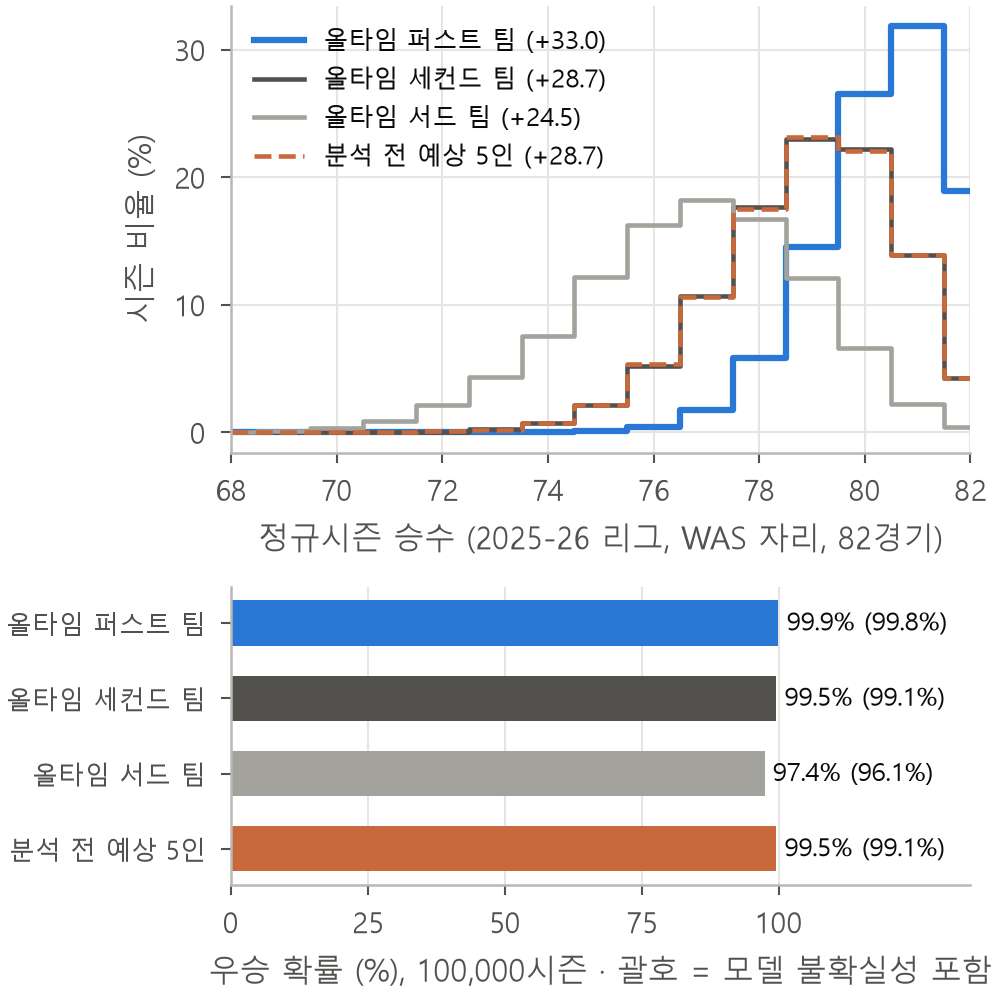
\includegraphics[width=\columnwidth]{fig11_all_time_season.png}
\caption{\LastSeason{} 리그 시뮬레이션 (팀당 \NSims{}시즌). 위: 정규시즌 승수 분포. 아래: 우승 확률 (괄호는 모델 불확실성 포함).}
\label{fig:alltimeseason}
\end{figure}

% =====================================================================
\section{역대 왕조 팀들과의 맞대결}\label{sec:dynasty}
여기서 끝내기는 조금 아쉬워서 역대 왕조 팀들과의 시뮬레이션도 시도해 보았습니다. 상대는 3점슛 시대의 대표 왕조 여섯 팀입니다: 1985--86 셀틱스, 1986--87 레이커스, 1995--96 불스, 2000--01 레이커스, 2013--14 스퍼스, 그리고 2016--17 워리어스입니다. 각 팀은 그 시즌의 실제 넷레이팅을 사용하며, 중립 경기장에서 단일 경기와 7전 4선승 시리즈를 각각 \NSims{}번 시뮬레이션하였습니다(수식~\eqref{eq:series}).\\

퍼스트 팀의 단일 경기 승률은 \FirstTeamDynGameMin{}--\FirstTeamDynGameMax{}였고, 가장 어려운 상대는 1995--96 불스였습니다(Figure~\ref{fig:dynasty}). 그래도 불스와의 시리즈 승률은 \FirstTeamBullsSeries{}이며, 서드 팀도 불스를 \ThirdTeamBullsSeries{}의 확률로 시리즈에서 이깁니다. 한 경기는 여전히 질 수 있지만(불스 상대 약 10번에 1번), 7전 4선승 시리즈에서는 거의 지지 않는다는 걸 볼 수 있습니다.\\

참고로 올타임 팀끼리 맞붙으면 퍼스트 팀은 세컨드 팀을 단일 경기 \FirstVsSecondGame{}, 시리즈 \FirstVsSecondSeries{}의 확률로 이기고, 서드 팀을 시리즈 \FirstVsThirdSeries{}의 확률로 이깁니다. 

\begin{figure}[t]
\centering
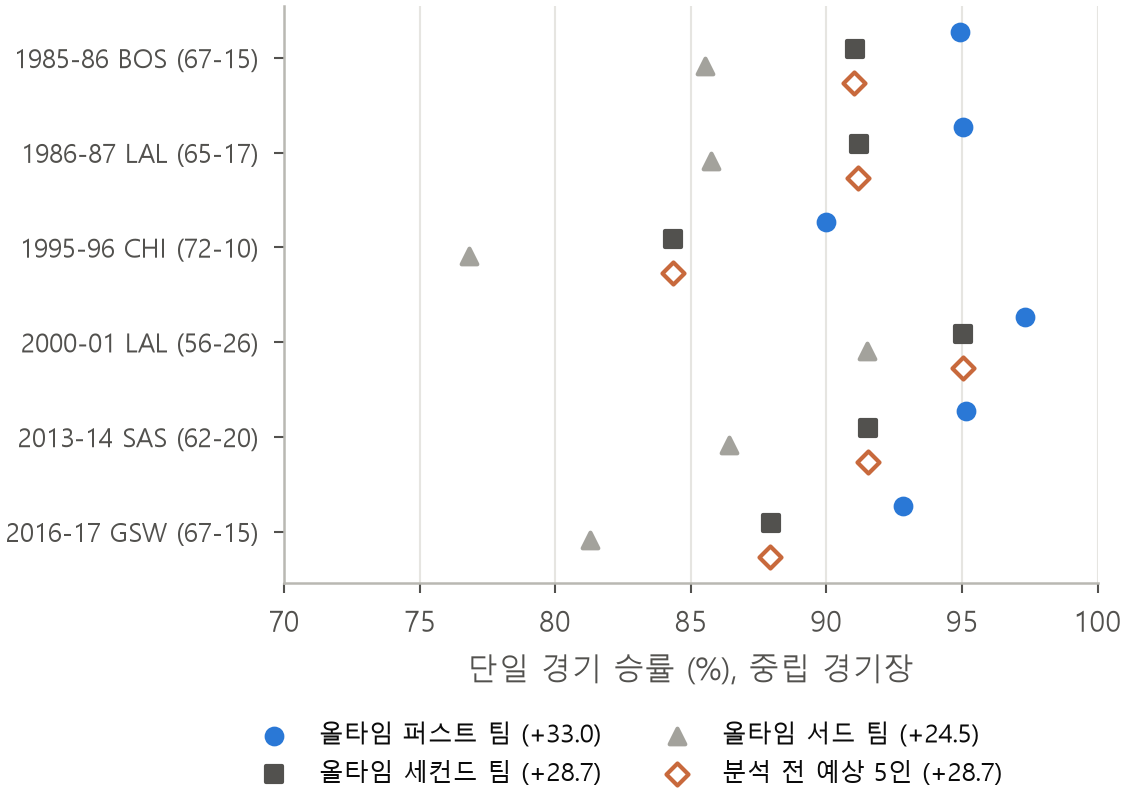
\includegraphics[width=\columnwidth]{fig12_all_time_dynasties.png}
\caption{올타임 팀과 역대 왕조 팀의 단일 경기 승률 (중립 경기장, 매치업당 \NSims{}회).}
\label{fig:dynasty}
\end{figure}

% =====================================================================
\section{분석 및 고찰}
분석을 시작하기 전 제 예상은 스테판 커리, 마이클 조던, 르브론 제임스, 래리 버드, 데이비드 로빈슨이었습니다. 이 다섯을 같은 방법으로 시뮬레이션하면(Table~\ref{tab:alltime}의 ``분석 전 예상 5인'') 넷레이팅 \PickTeamRating{}, 평균 \PickTeamWins{}승, 우승 확률 \PickTeamTitle{}로 세컨드 팀과 같은 수준이며, 퍼스트 팀과 맞붙으면 시리즈의 \FirstVsPickSeries{}에서 집니다. 제 예상과 다른 이유는 크게 세 가지입니다. 첫째, 니콜라 요키치가 전성기 BPM 1위로 센터 자리를 가져갔습니다. 둘째, 크리스 폴은 전성기 BPM이 커리와 같은 수준(+9.6)이면서 사용률이 낮고 수비 기여가 커서 다른 네 명과의 조합이 더 좋습니다. 셋째, 포워드 자리에서 야니스 아데토쿤보의 전성기 BPM(+10.5)이 버드(+9.0)보다 높았습니다.\\

화제가 된 82-0 게임 얘기로 다시 돌아가서 얘기를 조금 더 해보자면, 이 게임의 알고리즘은 각 선수의 득점·리바운드·어시스트·스틸·블록을 더한 점수로 시즌을 시뮬레이션하는데~\cite{game820}, 이는 본 연구의 검증에서 가장 부정확했던 박스스코어 합에 해당합니다. 또한, 제일 인기가 많은 NBA 2K 같은 경우에는 개발자가 정한 능력치를 씁니다. 마지막으로 스포츠 데이터사이언스 학계의 라인업 연구는 같은 시즌 실제 라인업의 성적을 예측하는 데 초점을 둡니다~\cite{nba2vec}. 제가 찾아본 범위에서는 정확도를 검증한 지표, 사용률 제약을 넣은 팀 모델, 올-NBA 방식의 전수 탐색, 시즌 전체 시뮬레이션을 함께 사용한 사례를 찾지 못하였습니다 (제가 한 연구가 어느 정도 독창적인 결과물이라는 걸 볼 수 있습니다!).

% =====================================================================
\section{한계}
이번 결과물의 몇 가지 한계들을 얘기하자면 (1) 1979--80 이후 선수만 다루므로 체임벌린, 러셀, 전성기의 압둘자바와 같은 과거의 선수들은 포함되지 않았습니다. (2) 다섯 명이 모든 경기의 모든 시간을 뛴다고 가정하여 부상, 피로, 벤치 선수를 고려하지 않았습니다. (3) 정규시즌 넷레이팅만 사용하므로, 2000--01 레이커스(플레이오프 15승 1패)처럼 플레이오프에서 더 강했던 팀은 과소평가됩니다. (4) 박스스코어는 수비를 거의 기록하지 못해 DBPM이 가장 약한 부분이며, 크리스 폴과 매직 존슨의 비교가 이 부분에 기대고 있습니다. (5) 포지션은 Basketball-Reference가 시즌마다 붙인 하나의 표기를 따르므로, 실제 역할과 다르게 표기된 선수가 있을 수 있습니다. (6) 각 선수의 BPM은 자기 시대의 리그 평균 대비 값이며, 이것이 다른 시대에도 그대로 통한다고 가정하였습니다. (7) 전성기는 가장 좋은 3시즌을 고른 것이므로 실제 실력보다 약간 높게 추정됩니다. (8) 사용률 합이 157\%인 실제 팀은 없으므로 모든 팀 모델은 데이터 밖을 외삽합니다. 그래디언트 부스팅~\cite{gbm}을 쓰면 퍼스트 팀의 우승 확률이 \BoostingTitleOdds{}로 크게 떨어지는데(Figure~\ref{fig:models}), 트리 기반 모델은 학습 데이터에서 보지 못한 입력에 대해 의미 있는 예측을 하지 못하기 때문입니다. (9) $k$는 비전공자가 이해하기 가장 어려운 개념이지만, 임의로 정한 값이 아니라 데이터에서 추정한 값이며, 90\% 구간(0.24--0.33) 안에서 $k$가 바뀌어도 퍼스트 팀의 넷레이팅은 1점 미만으로 바뀝니다.

\begin{figure}[t]
\centering
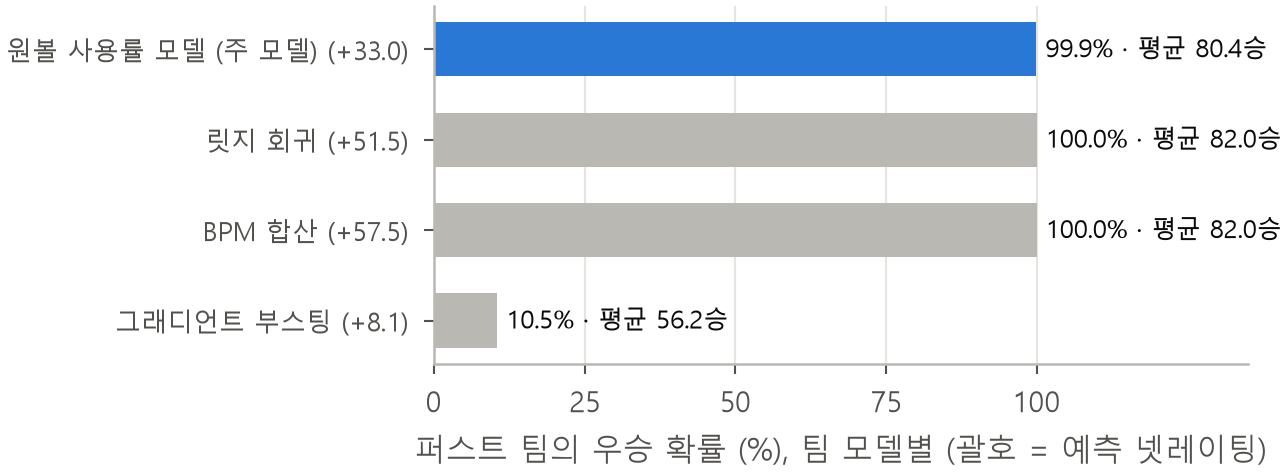
\includegraphics[width=\columnwidth]{fig13_model_sensitivity.png}
\caption{팀 모델에 따른 퍼스트 팀의 \LastSeason{} 우승 확률 (모델당 \NSims{}시즌). 괄호는 각 모델이 예측한 넷레이팅.}
\label{fig:models}
\end{figure}

% =====================================================================
\newpage
\section{결론}
본 연구는 1979--80 이후 NBA 데이터로 올-NBA 방식의 역대 최강 팀을 선정하였습니다. 퍼스트 팀은 \FirstTeamNames{}이며, 예측 넷레이팅 \FirstTeamRating{}으로 역대 최고의 실제 팀인 \BestRealTeam{}(\BestRealNR{})을 크게 앞서고, \LastSeason{} 시즌에서 \FirstTeamTitle{}의 확률로 우승합니다. 개인적으로 가장 큰 발견은 개인 기록의 합이 아니라 공 하나를 나눠 쓰는 조합이 결과를 좌우한다는 점입니다.\\

오늘날 스포츠는 통계와 시뮬레이션이 굉장히 중요합니다. 야구에서는 세이버메트릭스가 선수 평가를 바꾸었고, 오클랜드 애슬레틱스는 이를 활용해 적은 예산으로 경쟁력을 갖추었습니다~\cite{moneyball}. 포뮬러 1 팀들은 세이프티카나 고장 같은 무작위 사건을 몬테카를로 시뮬레이션으로 반영해 피트스톱 전략을 정합니다~\cite{f1mc}. NBA에서도 효율 분석이 3점슛 중심의 경기 방식으로의 변화를 이끌었습니다. 본 연구는 같은 도구를 작은 규모로 적용한 사례입니다.\\

제 진로는 스포츠 통계 분석이 아니지만, 전공에서 배운 데이터 처리, 검증, 탐색, 시뮬레이션을 오래 좋아해 온 농구에 적용해 본 즐거운 경험이었습니다. 수비를 더 정확히 반영하기 위해 플레이별 기록과 선수 추적 데이터를 쓰는 것은 향후 과제로 남깁니다.

% =====================================================================

\vspace{2\baselineskip}
\begin{thebibliography}{99}
\bibitem{bbref} Sports Reference LLC, ``Basketball-Reference.com: NBA and ABA history,'' \url{https://www.basketball-reference.com}, 2026.
\bibitem{bpm} D. Myers, ``About Box Plus/Minus (BPM),'' Basketball-Reference.com, 2020.
\bibitem{oliver} D. Oliver, \emph{Basketball on Paper: Rules and Tools for Performance Analysis}. Washington, DC: Potomac Books, 2004.
\bibitem{kubatko} J. Kubatko, D. Oliver, K. Pelton, and D. T. Rosenbaum, ``A starting point for analyzing basketball statistics,'' \emph{J. Quantitative Analysis in Sports}, vol. 3, no. 3, 2007.
\bibitem{sill} J. Sill, ``Improved NBA adjusted +/- using regularization and out-of-sample testing,'' in \emph{Proc. MIT Sloan Sports Analytics Conf.}, 2010.
\bibitem{ridge} A. E. Hoerl and R. W. Kennard, ``Ridge regression: Biased estimation for nonorthogonal problems,'' \emph{Technometrics}, vol. 12, no. 1, pp. 55--67, 1970.
\bibitem{gbm} J. H. Friedman, ``Greedy function approximation: A gradient boosting machine,'' \emph{Ann. Statist.}, vol. 29, no. 5, pp. 1189--1232, 2001.
\bibitem{kuhn} H. W. Kuhn, ``The Hungarian method for the assignment problem,'' \emph{Naval Res. Logist. Q.}, vol. 2, pp. 83--97, 1955.
\bibitem{mc} N. Metropolis and S. Ulam, ``The Monte Carlo method,'' \emph{J. Amer. Statist. Assoc.}, vol. 44, no. 247, pp. 335--341, 1949.
\bibitem{efron} B. Efron, ``Bootstrap methods: Another look at the jackknife,'' \emph{Ann. Statist.}, vol. 7, no. 1, pp. 1--26, 1979.
\bibitem{brier} G. W. Brier, ``Verification of forecasts expressed in terms of probability,'' \emph{Monthly Weather Review}, vol. 78, no. 1, pp. 1--3, 1950.
\bibitem{sklearn} F. Pedregosa \emph{et al.}, ``Scikit-learn: Machine learning in Python,'' \emph{J. Mach. Learn. Res.}, vol. 12, pp. 2825--2830, 2011.
\bibitem{game820} ABC7 Chicago, ``82-0? Pacers' Haliburton, Bucks, more get in on viral game,'' June 2026.
\bibitem{wis} Fox Sports, ``WhatIfSports 2015 NBA championship power rankings,'' 2015.
\bibitem{nba2vec} ``NBA2Vec: Dense feature representations of NBA players,'' arXiv:2302.13386, 2023.
\bibitem{moneyball} M. Lewis, \emph{Moneyball: The Art of Winning an Unfair Game}. New York: W. W. Norton, 2003.
\bibitem{f1mc} A. Heilmeier, M. Graf, J. Betz, and M. Lienkamp, ``Application of Monte Carlo methods to consider probabilistic effects in a race simulation for circuit motorsport,'' \emph{Applied Sciences}, vol. 10, no. 12, p. 4229, 2020.
\end{thebibliography}

\end{document}